
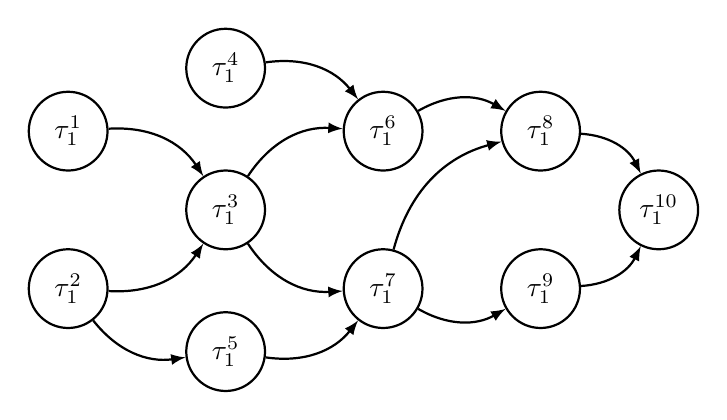
\begin{tikzpicture}[font={\fontsize{10pt}{12}\selectfont}]

\draw (0,1) node[circle, draw, thick, inner sep=0pt, minimum width=1cm] (t11) {$\tau_1^1$};
\draw (0,-1) node[circle, draw, thick, inner sep=0pt, minimum width=1cm] (t12) {$\tau_1^2$};

\draw (2,0) node[circle, draw, thick, inner sep=0pt, minimum width=1cm] (t13) {$\tau_1^3$};

\draw (2,1.8) node[circle, draw, thick, inner sep=0pt, minimum width=1cm] (t14) {$\tau_1^4$};
\draw (2,-1.8) node[circle, draw, thick, inner sep=0pt, minimum width=1cm] (t15) {$\tau_1^5$};

\draw (4,1) node[circle, draw, thick, inner sep=0pt, minimum width=1cm] (t16) {$\tau_1^6$};
\draw (4,-1) node[circle, draw, thick, inner sep=0pt, minimum width=1cm] (t17) {$\tau_1^7$};

\draw (6,1) node[circle, draw, thick, inner sep=0pt, minimum width=1cm] (t18) {$\tau_1^8$};
\draw (6,-1) node[circle, draw, thick, inner sep=0pt, minimum width=1cm] (t19) {$\tau_1^9$};

\draw (7.5,0) node[circle, draw, thick, inner sep=0pt, minimum width=1cm] (t110) {$\tau_1^{10}$};


\draw[-latex, thick, bend left] (t11) edge node {} (t13);
\draw[-latex, thick, bend right] (t12) edge node {} (t13);
\draw[-latex, thick, bend right] (t12) edge node {} (t15);

\draw[-latex, thick, bend left] (t14) edge node {} (t16);
\draw[-latex, thick, bend right] (t15) edge node {} (t17);

\draw[-latex, thick, bend left] (t13) edge node {} (t16);
\draw[-latex, thick, bend right] (t13) edge node {} (t17);

\draw[-latex, thick, bend left] (t16) edge node {} (t18);
\draw[-latex, thick, bend left] (t17) edge node {} (t18);
\draw[-latex, thick, bend right] (t17) edge node {} (t19);

\draw[-latex, thick, bend left] (t18) edge node {} (t110);
\draw[-latex, thick, bend right] (t19) edge node {} (t110);
\end{tikzpicture}
